\section{Introduction}\label{sec:introduction}
Finite-difference penalized least squares (PLS), developed from classical Whittaker graduation, extracts smooth trends from noisy observations while penalizing discrete variation \citep{whittaker1923,guerrero2007}. The nonnegative penalty $\lambda$ is mathematically natural, but identical numerical penalties need not produce comparable degrees of smoothing across difference orders or sample sizes. Guerrero's trace-based notion of smoothness \citep{guerrero2008} and its comparison with classical selection criteria by \citet{cortes2017} suggest an alternative: parameterize the same smoother by its normalized reduction in effective degrees of freedom.

Our focus is the bounded coordinate $s=S_d(\lambda)\in[0,1]$. Its endpoints represent interpolation and the degree-$(d-1)$ polynomial limiting trend, respectively. This is an exact change of coordinates for a published estimator, not a new estimator, loss function or guarantee of better optimization. A user can request $s$ while the numerical calculation internally evaluates $\lambda=S_d^{-1}(s)$.

The numerical literature already contains highly efficient Whittaker--Henderson and spline algorithms. \citet{weinert2007} develops specialized structural and GCV computations; related approaches exploit tensor-product structure and frequency-domain transformations \citep{eilers2006,garcia2010}. \citet{biessy2026} places Whittaker--Henderson smoothing in a modern statistical framework with Bayesian and computational extensions. Dense SVD cannot be characterized as universally faster than these structured methods. Our question is instead whether one spectrally consistent representation can make smoothness inversion, fitted curves, effective degrees of freedom and criterion evaluation reliable, particularly for high difference orders and extreme smoothness.

For a nonzero mean of the penalized differences, the usual affine formula constructs a degree-$d$ polynomial reference. This vector may become enormous even when the original observations are moderate, causing loss of floating-point accuracy. We derive a shift-free expression from the singular vectors of the difference operator that avoids this intermediate. It is tested against an independent 85-digit reference, with numerical failures retained in the analysis rather than silently discarded.

A second issue concerns the residual-based BIC expression studied by \citet{cortes2017}: as smoothing approaches interpolation, the residual sum of squares shrinks quadratically in $\lambda$, so this BIC diverges to negative infinity. We prove the limit, record it as a limitation of the unrestricted criterion and evaluate two explicitly constrained candidate ranges. Finally, a small simulation compares established criteria using the true latent trend, not a fitted residual or a future forecast.

We contribute (i) a unified smoothness-indexed SVD formulation and a shift-free identity for fitting; (ii) a numerical-validation study with independent multiprecision reference solutions; (iii) an explicit analysis of the BIC interpolation boundary; and (iv) reproducible pilot evidence on true trend-recovery error. Full spectral SVD is adopted as an accuracy-oriented default for the proposed framework, while its dense computational cost and remaining prior-art benchmarks are acknowledged. Figure~\ref{fig:map} illustrates why the internal penalty depends strongly on the difference order.

\begin{figure}[t]
\centering
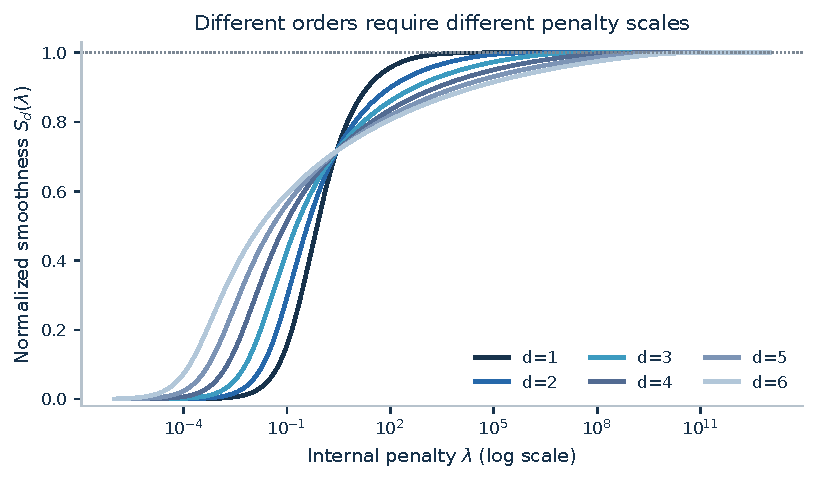
\includegraphics[width=\columnwidth]{figures/smoothness_map.pdf}
\caption{Normalized smoothness against the internal penalty for $n=64$ and orders $d=1,\ldots,6$. Different orders have different penalty scales even at equal normalized conditional smoothness. Curves are constructed from the positive singular spectrum, independently of any observed series.}
\label{fig:map}
\end{figure}
